\documentclass[../besoin_user.tex]{subfiles}
\begin{document}

\section{Menu principal}
\begin{figure}[h]
    \centering
    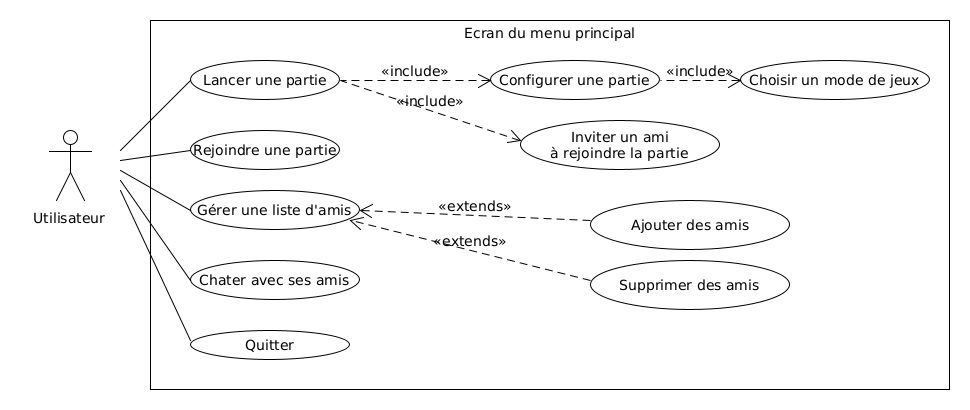
\includegraphics[scale=0.5]{img_fonctionnel/use_case_user_ecran_principal.png}
    \label{fig:user_menu_principal}
    \caption{Menu principal}
\end{figure}

Le menu principal est la première interface que l'utilisateur voit lorsqu'il lance le jeu.
Elle reprend les informations suivantes:
\begin{itemize}
    \item[-] La liste des amis
    \item[-] Les notifications (si l'utilisateur a reçu un message)
    \item[-] Les différents menus accessibles depuis l'écran principal 
\end{itemize}

\subsection{Lancement d'une partie}
Lors du lancement d'une partie le joueur doit simplement fixer les règles en choisissant :
\begin{itemize}
	\item[-] Le type de partie : \textbf{classique} ou \textbf{commandant}
	\item[-] Le temps d'une partie : au maximum \textbf{15 minutes}
	\item[-] Le temps par tour d'un joueur : au maximum \textbf{30 secondes}
\end{itemize}

Après quoi il sera redirigé vers un lobby, auquel il pourra inviter des joueurs, qui seront tous en mode spectateur s'ils acceptent l'invitation.
Un joueur peut aussi rejoindre le lobby sans recevoir d'invitation.
Si au moins un joueur à rejoint la partie, le joueur principale peut le fixer en tant que second joueur et lancer la partie.
Mais avant que la partie ne puisse commencer, il faudra placer tous les bateaux disponibles sur le board, après quoi la partie se lance.

\subsection{Rejoindre une partie}
Afin de rejoindre une partie, l'utilisateur doit simplement entrer un code de partie qu'il aura reçu de la part du joueur principal.
Notons que le code peut être envoyé par le biais du chat, ou tout autre moyen de communication.

\subsection{Gérer sa liste d'ami}
Chaque utilisateur possède une liste d'amis qu'il peut modifier. Il a la possibilité de:
\begin{itemize}
    \item ajouter un ami a sa liste
    \item retirer un ami de sa liste
\end{itemize}
La liste d'ami permet d'initier chat avec l'ami, ce qui permet de notamment communiquer avec lui, mais également de lui envoyer des codes de partie.

\subsection{Chat}
Si le joueur a des amis en ligne dans sa liste d'amis, il a la possibilité de communiquer avec eux via un chat. 
Si le joueur n'est pas en ligne, il peut tout de même envoyer un message, qui sera reçu par l'ami lorsqu'il se connectera.
Cependant, nous ne pouvons pas assurer le système de notification lorsque l'ami n'est pas en ligne.

\end{document}